\section{dReach: System Description}
\begin{figure}
  \centering
  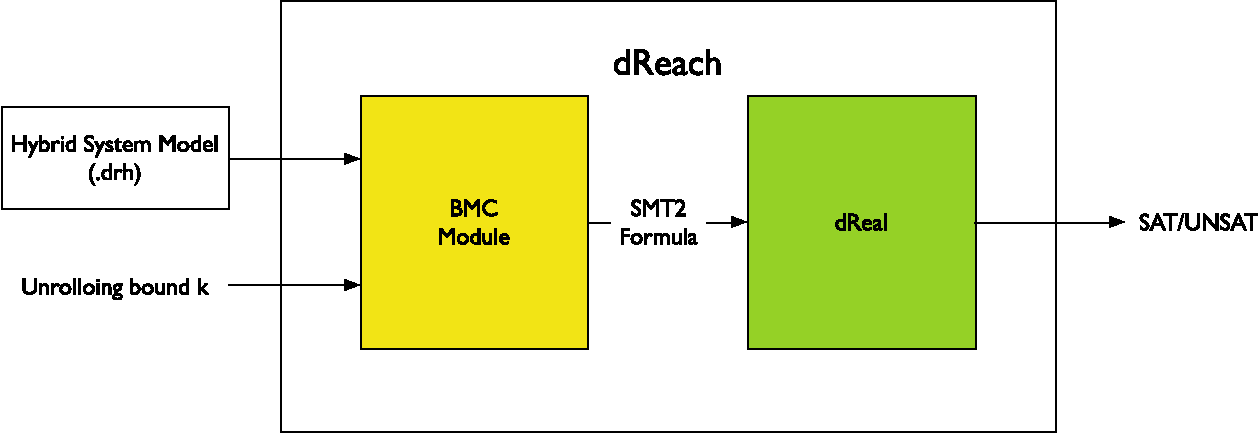
\includegraphics[width=\textwidth]{images/dReach}
  \caption{System Description of \dReach{}}
  \label{fig:system-description}
\end{figure}

Figure~\ref{fig:system-description} illustrates the architecture of
\dReach{}. We provide a domain-specific lanaguage to describe a hybrid
system and specify its safety properties. Given an input model,
specification, and unrolling bound $k$, \dReach{} reduces the
$\delta$-reachability problem to a $\delta$-decision problem of
formulas over the reals by providing a corresponding SMT encoding for
the problem. Then, the bounded reachability queries are answered by
using our nonlinear SMT solver \dReal{}~\cite{DBLP:conf/cade/GaoKC13}.

\subsection{drh: a Language for Modeling and Specifying Hybrid Systems}

We define \texttt{drh}, a language for describing hybrid systems and
specifying their safety conditions. It consists of five sections -
macro definitions, variable declarations, mode definitions, and
initial condition, and goals.
\begin{align*}
  \textit{drh} := \ & \textit{macro-definition}^*\\
                    & \textit{variable-declaration}^+\\
                    & \textit{mode-definition}^+\\
                    & \textit{initial-condition}\\
                    & \textit{goal}^+
\end{align*}
In macro definitions, we allow users to define macros in
C preprocessor (\texttt{cpp}) style which can be used in following
sections. Macro expansions occur before the other parts are processed.

A variable declaration has a form:
\[
\textit{variable-declaration} \ := \ \texttt{[}
                                     \textit{l}
                                     \texttt{,}
                                     \ \textit{u}
                                     \texttt{]}
                                     \ \textit{var}
                                     \texttt{;}
\]
and it declares a real variable, $var$, whose domain is an Real
interval $[l, u] \in \mathbb{IR}$. It requires a variable declaration
for a special variable, \textit{time}, to specify the upperbound of
time duration in the analysis of bounded reachability.

A mode definition consists of mode id, mode invariant, flow, and jump.
\begin{align*}
  \textit{mode-definition} \ := & \ \texttt{\{}
                                    \texttt{mode} \ \textit{id}\texttt{;}\\
                           & \ \ \  \texttt{invt}:(\textit{formula} \texttt{;})^+\\
                           & \ \ \  \texttt{flow}:\textit{ode}^+\\
                           & \ \ \ \texttt{jump}:\textit{jump}^+ \texttt{\}}
\end{align*}
\textit{id} is a unique positive interger assigned to a mode. An
invariant is a conjuction of logic formulae which must always hold in
a mode. A flow describes a continuous dynamics of a mode by providing
a set of ordinary differential equations (\textit{ode}s) which is a
form of
``\texttt{d/dt[}\textit{x}\texttt{]=}\textit{exp}''. \textit{jump} is
a form of ``\textit{guard} \texttt{==>} \texttt{@}\textit{n}
\textit{reset}'' where \textit{guard} is a logic formula specifying a
condition to make a transition, $n$ denotes the target mode-id, and
\textit{reset} is a logic formula connecting the old and new values
for the transition.

\texttt{initial-condition} is of a form
``\texttt{@}\textit{mode-id} \textit{formula}\texttt{;}''
where \textit{mode-id} is an initial mode of a hybrid system and
\textit{formula} specifies the initial configuration of it.

\texttt{goal} shares the same syntactic structure,
``\texttt{@}\textit{mode-id} \textit{formula}\texttt{;}'' of
\textit{initial-condition} with a different interpretation. It poses a
reachability question: ``Is there a trajectory of a hybrid system
reaching \textit{mode-id} while satisfying the goal condition \textit{formula}?''.

\subsection{Encoding Bounded Reachability Problem}

Our previous work~\cite{DBLP:journals/corr/GaoKCC14} already studied
logic encodings of bounded reachability problems of hybrid
systems. The encoding scheme is based on the standard bounded model
checking while non-trivial mode invariants and systems with
nondeterministic flows make the problem interesting.

In this section, we explain the extensions and variable naming
convention that we make to the standard SMT-LIB~\cite{BarST-SMT-10} to
represent flows and mode invariants of hybrid systems.

\paragraph{Variable naming convention}
In our encoding, a system variable $\texttt{x\_i\_p}$ has two
subscripts $i \in \mathbb{N}$ and $p \in \{0, t\}$. The first
subscript $i$ indicates that it represents the value of a system
variable $x$ at the $i$-th step. The second subscript $p \in \{0, t\}$
denotes the value at the begining of mode (end of mode,
respectively). For instance, $x\_0\_t$ denotes the value of variable
$x$ at the end of first mode (step 0).

\paragraph{\texttt{define-ode} and \texttt{integral}}
Many hybrid systems formulate their flows implicitly using
the Picard-Lindel$\ddot{o}$f representation:
\[
[x\_1\_t, x\_2\_t, \dots, x\_n\_t] = \int_0^t \vec{g}([x_1(s), x_2(s), \cdots,
x_n(s)]) \mathrm{d}s.
\]
In \dReach~{}, we use \texttt{define-ode} to name a flow by assigning
a name to it. Then \texttt{integral} connects the value of the initial
and final variables. For instance, the following example

\begin{Verbatim}[fontfamily=courier]
(define-ode flow_1 ((= d/dt[x] v) (= d/dt[v] -9.8)))
(integral 0 time_0 [x_0_0 v_0_0] flow_1)
\end{Verbatim}

defines a flow $\dot{x} = \int_0^t v(s) \mathrm{d}s$ and $\dot{v} =
\int_0^t -9.8 \mathrm{d}s$ and assigns a name $\mathit{flow_1}$ to it.
Command \texttt{integral} establish the relationship between the value
of varialbes at the beginning of a mode and at the end of it.

\paragraph{\texttt{forall\_t}}
\begin{Verbatim}[fontfamily=courier]
(forall_t 2 [0 time_3] (>= x_3_t 0))
\end{Verbatim}

%%% Local Variables:
%%% mode: latex
%%% TeX-master: "main"
%%% End:
